\section{Bonding, Formula and Nomenclature}

\begin{multicols}{2}


\section*{Valence and Chemical \hfill \\ Formulae} \index{Valence} \index{Ions} \index{Chemical formulae}


\subsection{Student Ions}

\begin{center}
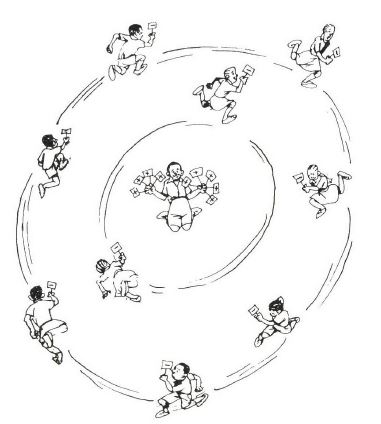
\includegraphics[width=0.49\textwidth]{./img/source/student-ions.jpg}
\end{center}

\begin{description*}
%\item[Subtopic:]{}
\item[Materials:]{Cards/paper, students}
\item[Setup:]{Label many cards with symbols to represent subatomic particles (`+' for protons, `-' for electrons, blank for neutrons).}
\item[Procedure:]{Place one chair in a large room to represent a nucleus. Then place chairs in circles around the centre to represent energy levels of electrons - 2 in the first cirlce, then 8, etc. Have 1 student sit in the middle chair and others in the outer chairs to represent electrons in an atom. Do this for two atoms, e.g. sodium and chlorine. Note that neither atom has a full outer shell. Have students move from one atom to the other in order to fill the outermost shells. }
%\item[Hazards:]{}
%\item[Questions:]{}
%\item[Observations:]{}
\item[Theory:]{One atom (often a metal) loses electron(s) and another (usually non-metal) gains electron(s). This results in positively and negatively charged \emph{ions}.}
%\item[Applications:]{}
\item[Notes:]{Adapt this for covalent bonds as well, having students from each atom move to represent shared electrons.}
\end{description*}

\columnbreak

\subsection{Ionic Formula Templates}

\begin{center}
%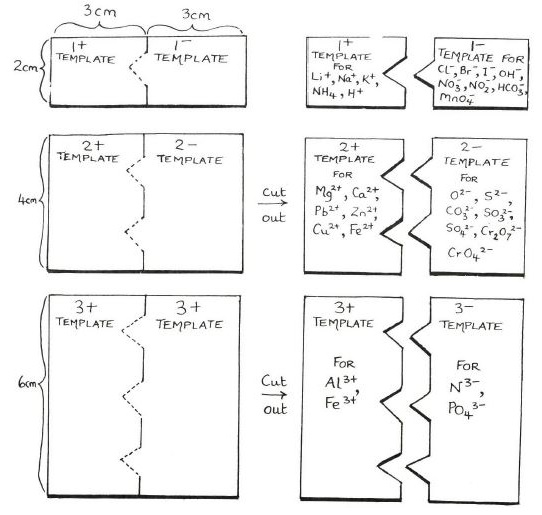
\includegraphics[width=0.49\textwidth]{./img/source/ion-template.jpg}
%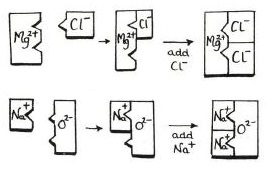
\includegraphics[width=0.49\textwidth]{./img/source/ion-template-2.jpg}
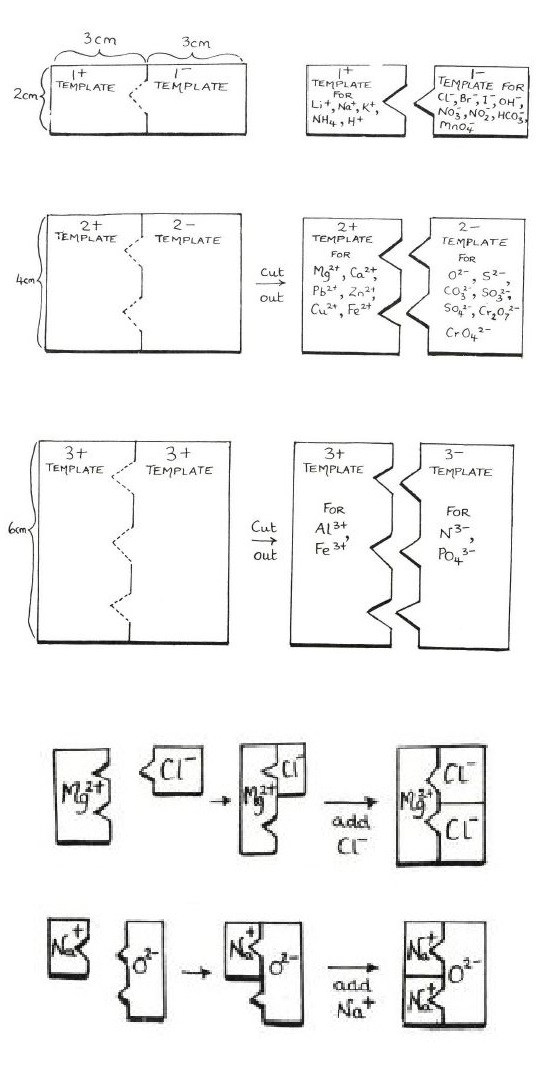
\includegraphics[width=0.49\textwidth]{./img/source/ion-templates.jpg}
\end{center}

\begin{description*}
%\item[Subtopic:]{}
\item[Materials:]{Cardboard, scissors, markers}
%\item[Setup:]{}
\item[Procedure:]{Cut out templates for different ions as shown. Use them to make different molecule combinations and then write their chemical formulae based on the templates.}
%\item[Hazards:]{}
%\item[Questions:]{}
%\item[Observations:]{}
%\item[Theory:]{}
%\item[Applications:]{}
%\item[Notes:]{}
\end{description*}

\vfill
\columnbreak

%==================================================================================================%

%\section*{Valence}


\subsection{Valencies Ruler}

\begin{center}
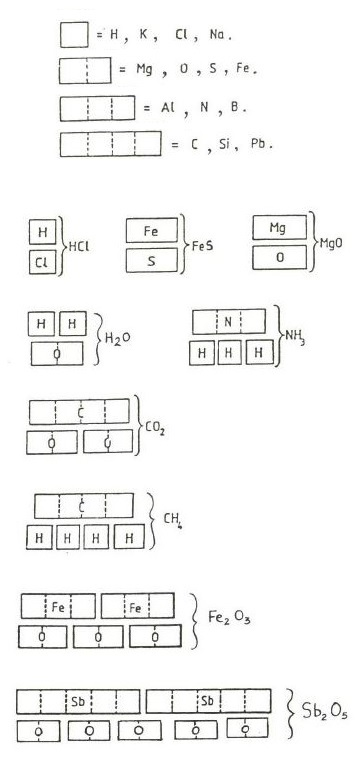
\includegraphics[width=0.49\textwidth]{./img/source/valency-ruler.jpg}
\end{center}

\begin{description*}
%\item[Subtopic:]{}
\item[Materials:]{Cardboard, scissors, markers}
%\item[Setup:]{}
\item[Procedure:]{Measure and cut strips of paper or cardboard as shown in the figure (valency 1 represented by
l cm $\times$ 1 cm card, valency 2 by l cm $\times$ 2 cm card,
valency 3 by 1 cm $\times$ 3 cm etc). Write chemical
symbols on the strips. For blackboard figure
demonstrations the strips can be bigger.}
%\item[Hazards:]{}
%\item[Questions:]{}
%\item[Observations:]{}
\item[Theory:]{The valency of an element gives the number of
hydrogen atoms which that element can bond to or
replace. For example, Group I elements have a valency of 1, and group VI elements such as sulphur have a valency of $8-2=6$.}
%\item[Applications:]{}
%\item[Notes:]{}
\end{description*}

\vfill
\columnbreak

%==================================================================================================%

\section*{Chemical Bonding} \index{Bonding}


\subsection{Covalent Bonds}

\begin{center}
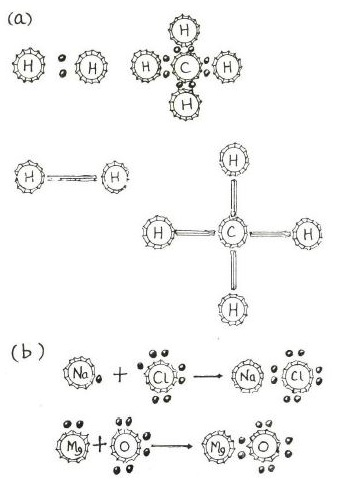
\includegraphics[width=0.43\textwidth]{./img/source/covalent-bonds.jpg}
\end{center}

\begin{description*}
%\item[Subtopic:]{}
\item[Materials:]{Bottle caps, matches, peas/seeds}
%\item[Setup:]{}
\item[Procedure:]{Break the heads off of many matches. A pair of electrons in a covalent bond may be
represented by a matchstick without a  head, while the heads can be used to represent electrons (a). Ionic bonds can be represented by bottle caps
and match heads or stones/seeds as well (b).}
%\item[Hazards:]{}
%\item[Questions:]{}
\item[Observations:]{It can be seen that the covalent bonds often fill the outermost energy level for the atoms, thus making the arrangement more stable.}
\item[Theory:]{In covalent bonds, one or more electrons are shared between atoms.}
%\item[Applications:]{}
%\item[Notes:]{}
\end{description*}

\subsection{Student Bonding}

%\begin{center}
%\includegraphics[width=0.4\textwidth]{./img/.jpg}
%\end{center}

\begin{description*}
%\item[Subtopic:]{}
\item[Materials:]{Paper, students}
%\item[Setup:]{}
\item[Procedure:]{Give each student a sheet of paper with a different ion written on it. For example, give 1 student a paper reading `Fe$^{3+}$' and 3 others papers reading `Cl$^-$'. Have the students run around randomly to represent being in an unstable state. Then have them all come together to form a stable molecule of FeCl$_3$.}
%\item[Hazards:]{}
%\item[Questions:]{}
%\item[Observations:]{}
%\item[Theory:]{}
%\item[Applications:]{}
%\item[Notes:]{}
\end{description*}

\subsection{Molecule Models} \index{Molecules} % Source 114

\begin{center}
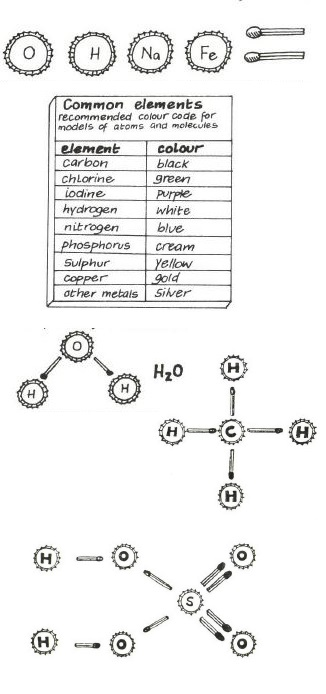
\includegraphics[width=0.45\textwidth]{./img/vso/molecule-model.jpg}
\end{center}

\begin{description*}
%\item[Subtopic:]{}
\item[Materials:]{Bottle caps, matches}
%\item[Setup:]{}
\item[Procedure:]{Mark the bottle caps with a pen or marker. Matchsticks form the bonds. Colour the bottle caps according to the recommendations given to represent different elements. Try to make all the examples in your textbook.}
%\item[Hazards:]{}
%\item[Questions:]{}
%\item[Observations:]{}
%\item[Theory:]{}
%\item[Applications:]{}
%\item[Notes:]{}
\end{description*}

\vfill
\columnbreak

\subsection{3-D Models}

\begin{center} % Source 125
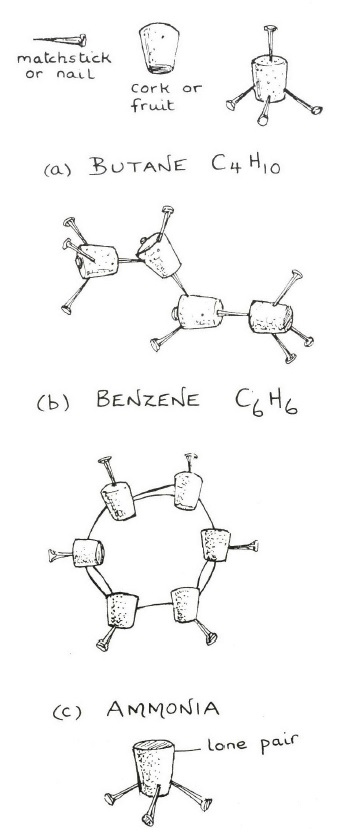
\includegraphics[width=0.43\textwidth]{./img/source/3d-models-2.jpg}
\end{center}

\begin{description*}
%\item[Subtopic:]{}
\item[Materials:]{Cork, nails}
%\item[Setup:]{}
\item[Procedure:]{Use this alternative method for 3-dimensional models of molecules. Nails can represent hydrogen atoms and the corks carbon.}
%\item[Hazards:]{}
%\item[Questions:]{}
%\item[Observations:]{}
%\item[Theory:]{}
%\item[Applications:]{}
%\item[Notes:]{}
\end{description*}

\vfill
\columnbreak

\subsection{Additional Model Ideas}

\begin{center}
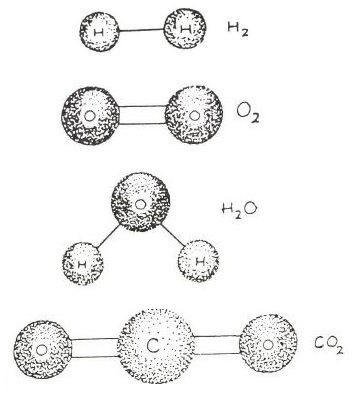
\includegraphics[width=0.43\textwidth]{./img/source/3d-models.jpg}
\end{center}

\begin{description*}
%\item[Subtopic:]{}
\item[Materials:]{Small round objects (e.g. fruits, seeds, cork, foam pieces), wire/string/sticks/matches}
%\item[Setup:]{}
\item[Procedure:]{Use the wire, string, etc. for the bonds and the fruits etc. for the atoms. Use the same colour-coding as mentioned above.}
%\item[Hazards:]{}
%\item[Questions:]{}
%\item[Observations:]{}
%\item[Theory:]{}
%\item[Applications:]{}
%\item[Notes:]{}
\end{description*}

\vfill
\columnbreak

\subsection{Model Box} \index{Storage}

\begin{center}
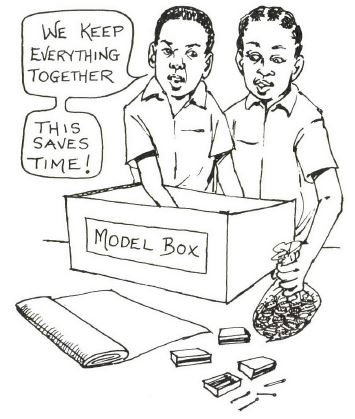
\includegraphics[width=0.4\textwidth]{./img/source/model-box.jpg}
\end{center}

\begin{description*}
%\item[Subtopic:]{}
\item[Materials:]{Cardboard box, bottle caps, matches, seeds/peas/etc.}
%\item[Setup:]{}
\item[Procedure:]{Create a model box for students to use when making models of atoms, molecules, etc.}
%\item[Hazards:]{}
%\item[Questions:]{}
%\item[Observations:]{}
%\item[Theory:]{}
%\item[Applications:]{}
%\item[Notes:]{}
\end{description*}


\end{multicols}


\pagebreak